
\documentclass[conference]{IEEEtran}
\usepackage{fancyhdr}
\usepackage{graphicx}
\usepackage{listings}
\usepackage{caption}
\usepackage{algorithm}
\usepackage{textcomp}
\usepackage{algpseudocode}
\usepackage{amssymb}
\usepackage{cite}
\usepackage{multirow}
\usepackage{verbatim}
\usepackage{subcaption}
\usepackage{enumerate}   

\usepackage[colorlinks,
linkcolor=red,
anchorcolor=black,
citecolor=black
]{hyperref}
\hyphenation{op-tical net-works semi-conduc-tor}

\newcommand{\jin}[1]{\textcolor{blue}{{\it [jin add: #1]}}}



\begin{document}
\pagestyle{plain}	
%
% paper title
% can use linebreaks \\ within to get better formatting as desired
\title{Empirical Study of Just-in-Time Prediction of Performance Regression Introducing Change}

% author names and affiliations
% use a multiple column layout for up to two different
% affiliations

\author{\IEEEauthorblockN{Kundi Yao, Jinfu Chen}
\IEEEauthorblockA{Department of Software Engineering \\
Concordia University\\
Montreal, Canada\\
email: \{ku\_yao,fu\_chen\}@encs.concordia.ca}
}
% make the title area
\maketitle
\begin{comment}


\begin{abstract}
Performance is an important aspect of software quality. Performance issues may compromise user experiences, increase the operating cost of the system, and cause field failures. In fact, large software systems failures are often due to performance issues rather than functional bugs. One of the most prevalent performance issues is performance regression. Examples of performance regressions are response time degradation and higher than before resource utilization. Although prior research proposes various automated approaches that detect performance regressions, the detection is conducted after fact, i.e., after the system is built and deployed in the field or dedicated performance testing environments. On the other hand, there exists rich software quality research that examines the impact of code changes on software quality; while majority of prior findings do not use performance regression as a sign of software quality degradation. In this paper, we perform an exploratory study on the source code changes that introduce performance regressions. We conduct a statistically rigorous performance evaluation on 376 commits from two releases of \emph{Hadoop} and 135 commits from five releases of \emph{RxJava}. In particular, we identify performance regressions in each commit if there exists statistically significant and non-trivial performance degradation, in terms of either response time, CPU usage, Memory usage or I/O traffic, compared to the last commit. By manually examining the JIRA issue reports that are associated with the identified performance regression introducing commits, we find that the majority of the performance regressions are introduced while fixing other bugs. In addition, we find that most of such regressions are due to expensive function calls. Our findings suggest that developers may introduce performance regressions when completing code changing tasks without considering the impact on performance. Automated tooling support can be proposed to help developers be aware of the possible performance impact while changing source code.

\end{abstract}

\begin{IEEEkeywords}
Performance Regression; Code Changes; Mining Software Repositories
\end{IEEEkeywords}

\end{comment}

% For peer review papers, you can put extra information on the cover
% page as needed:
% \ifCLASSOPTIONpeerreview
% \begin{center} \bfseries EDICS Category: 3-BBND \end{center}
% \fi
%
% For peerreview papers, this IEEEtran command inserts a page break and
% creates the second title. It will be ignored for other modes.
\IEEEpeerreviewmaketitle

\section{Introduction}
% no \IEEEPARstart
\label{sec:intro}

The rise of large-scale software systems (e.g., Amazon.com and Google Gmail) has posed an impact on people's daily lives from mobile devices users to space station operators. The increasing importance and complexity of such systems makes their quality a critical, yet extremely difficult issue to address. Failures in such systems are more often associated with performance issues, rather than with feature bugs~\cite{Weyuker:2000}. Therefore, performance assurance activities are an essential step in the release cycle of large software systems. 

Performance assurance activities aim to identify and eliminate performance regressions in each newly released version. Examples of performance regressions are response time degradation, higher than expected resource utilization and memory leaks. Such regressions may compromise the user experience, increase the operating cost of the system, and cause field failures. The slow response time of the United States' newly rolled-out healthcare.gov illustrates the importance of performance assurance activities before releasing a system. Failure in detecting such regressions would result in significant financial and reputational repercussions.

Prior software quality research typically focus on functional bugs rather performance issues. For example, post-release bugs are often used as code quality measurement and are modelled by statistical modeling techniques in order to understand the relationship between different software engineering activities and code quality~\cite{Hassan:2009:PFU}. In addition, bug prediction techniques are proposed to prioritize software quality assurance efforts~\cite{Zimmermann:2007:PDE,Nagappan:2005:URC,Nagappan:2006:MMP} and assesses the risk of code changes~\cite{emadjit}. However, performance regressions are rarely targeted in spite of their importance.

On the other hand, prior study of JIT defect prediction focus more on the risk of commit haved a bug rather than performance regressions. Predicting performance regressions remains a task that is conducted after fact, i.e., after the system is built and deployed in the field or dedicated performance testing environments. However, large amounts of resources are required to detect, locate, understand and fix performance regressions at such a late stage in the development circle; while the amount of required resources would be significantly reduced if developers were notified whether a code change introduces performance regressions during development. 

In this research, we perform an empirical study on the JIT prediction of performance regression introducing code changes. 
By examining the identified performance regression introducing changes, we find that performance regression introducing changes are prevalent during software development. The identified performance regressions are often associated with complex syndrome, i.e., multiple performance metrics have performance regression. In order to build a change risk model to predict JIT performance regression, we combine the basic commit-level measures proposed by Mockus and Weiss \cite{mockus2000predicting}, which are based on the characteristics of code changes, such as the number of modified subsystems and the purpose of the code change with the performance related measures we added, such as changing conditions and passing expensive parameters.

%Interestingly, we find that performance regression introducing changes also improve performance at the same time. Such results show that developers may not be aware of the existence of performance regressions, even when they are trying to improve performance. By studying the context and root-causes of performance regression introducing changes, we find that performance regressions are mostly introduced while fixing other functional bugs. We identify six code level root-causes of performance regressions, where majority of the performance regressions are introduced due to adding expensive function calls.

%Our study results shed light on the characteristic of performance regression introducing changes and suggest the lack of awareness and systematic performance regression testing in practice. Based on our findings, performance-aware change impact analysis and designing inexpensive performance tests may help practitioners better mitigate the prevalent performance regression that are introduced during software development.

The rest of this proposal is organized as follows: Section~\ref{sec:related} presents the prior research that is related to this project. Section~\ref{sec:case} presents our subject systems and our approach of predicting performance regression introducing code changes. Section~\ref{sec:results} presents our research questions. Finally, Section~\ref{sec:milestones} presents the milestones for the project.



\section{Related Work}
\label{sec:related}
In this section, we present the related prior research to this paper in three aspects: 1) current state-of-the-art performance regression detection, 2) Prediction of JIT software defect and 3) empirical study on performance.

%\subsection{Motivation}
%As software evolves problematic code changes can significantly degrade software performance. Performance regression affects the quality and use of software so we have to find the root cause of problematic code change and fix the performance bugs. Performance regression testing can detect the bugs but the testing is resource consuming and high cost. The goal of our research is to detect the code changes which cause performance regression and classify what kind of performance bug the problematic codes cause. At the same time, we need improve performance regression testing efficiency through skip non-regressing commits and test case reduction.
\subsection{Performance regression detection}
A great amount of research has been proposed to detect performance regression.

Ad hoc analysis selects a limited number of target performance counters (e.g., CPU and memory) and performs simple analysis to compare the target counters. Heger et al.~\cite{Heger:2013:ARC} present an approach to support software engineers with root cause analysis of the problems. Their approach combines the concepts of regression testing, bisection and call tree analysis to detect performance regression root cause analysis as early as possible.

Pair-wise analysis compares and analyzes the performance metrics between two consecutive versions of a system to detect the problem. Nguyen et al.~\cite{Nguyen:2012:ADP,nguyen2011automated,Nguyen:2014:ICS} conduct a series of studies on performance regressions. Nguyen et al. propose an approach to detect performance regression by using a statistical process control technique called control charts. They construct the control chart and apply it to detect performance regressions and examine the violation ratio of the same performance counter. Malik et al.~\cite{Malik:2013:ADP} propose approaches that combine one supervised and three unsupervised algorithms to help performance regression detection. They employ feature selection methods named Principal Component Analysis (PCA) to reduce the dimensionality of the observed performance counter set and validate their approach through a large case study on a real-world industrial software system~\cite{malik2010automatic}.

Model-based analysis builds a limited number of detected models for a set of target performance counters (e.g., CPU and memory) and leverages the models to detect performance regressions. 
Xiong et al.~\cite{Xiong:2013:VAM} propose a model-driven framework to diagnose the application performance in cloud condition without manual operation. In the framework, it contains three modules consisted of sensor module, model building module and model updating module. It can automatically detect the workload changes in cloud environment and lead to root cause of performance problem. Cohen et al.~\cite{cohen2004correlating} propose an approach that builds  a promising class of probabilistic models (Tree-Augmented Bayesian Networks or TANs)  to correlate system level counters and systems’ average-case response time. Cohen et al.~\cite{Cohen:2005:CIC} present that performance counters can successfully be used to construct statistical models for system faults and compact signatures of distinct operational problems. Bodik et al.~\cite{bodik2008hilighter} employ logistic regression with L1 regularization models to construct signatures to improve Cohen et al.\textquotesingle s work.

Multi-models based analysis builds multiple models from performance counters and uses the models to detect performance regressions. Foo et al.~\cite{foo2010mining} propose an approach to detect potential performance regression using association rules. They utilize data mining to extract performance signatures by capturing metrics and employ association rules techniques to collect correlations that are frequently observed in the historical data. Then use the change to the association rules to detect performance anomalies. Jiang et al.~\cite{jiang2009automatic} present two diagnosis algorithms to locate faulty components: RatioScore and SigScore based on component dependencies. They identify the strength of relationships between metric pairs by utilizing an information-theoretic measures  and track system state based on in-cluster entropy. A significant change in the in-cluster entropy is considered as a sign of a performance fault. Shang et al.~\cite{Shang:2015:ADP} propose an approach that first clusters performance metric based on their correlation. Each cluster of metrics is used to build statistical model to detect performance regressions. 

Prior research on performance regressions are designed to be conducted after the system is built and deployed in either performance testing environments or user environments. In this paper, we explore performance regression at commit level, i.e., when the performance regressions are introduced into the software. 

\subsection{Prediction of JIT software defect}
Kamei et al.~\cite{Kamei2013TSE}  present some change measures and builds a logistic regression model to predict just-in-time software defect. The change measures consist of 14 factors derived from six open-source projects and five commercial projects and are grouped into five dimensions. The prediction model the paper builded is able to predict defect-inducing changes with 68 percent accuracy and 64 percent recall. The finding also shows that which part of the factors play more important role in defect-inducing changes. Compared with this paper, we add another factors related performance regression to build the prediction model. Another is that this paper utilizes SZZ algorithm to identify whether or not a change will introduce a defect. However, if the repository does not report the defect we cannot map the defect back to the defect-inducing change. Fukushima et al.~\cite{Fukushima:2014:ESJ} construct Just-in-Time defect prediction cross-project models to identify source code changes that have a high risk of introducing a defect. Zhang et al.~\cite{Zhang:2014:TBU}build a universal defect prediction model for a large set of projects by combining context factors and clustering similar projects to determine the different software metrics sets. In order to find whether or not unsupervised models perform better than the supervised models in effort-aware just-in-time defect prediction, Yang et al.~\cite{Yang:2016:EJD} consider fourteen change metrics and build simple unsupervised and supervised models to predict software defect to determine whether they are of practical value. The results show that many simple unsupervised models perform better than the state-of-the-art supervised models in effort-aware just-in-time defect prediction. Shivaji et al.~\cite{Shivaji2013TSE} realise that the more features (factors) prediction model learned, the more insufficient performance the model predicts, so they perform multiple feature selection algorithms to reduce the factors to predict software bug in a high performance. For the purpose of reducing the number of software failures, Mockus and Weiss ~\cite{mockus2000predicting} are the first one to utilize a number of change measures to build linear regression to predict the probability of failure for a software change. Such change measures include size, duration, diffusion, and type, as well as the experience of the developers who implemented it. However, the discovered defect-inducing changes may be incomplete, which is a potential threat to the correctness of the prediction model. Kamei et al.~\cite{kamei2016studying} construct JIT model based on cross-project models, by using larger pool of training data and combining models from other projects to establish their JIT models, and the result shows performance of within-project model outperforms cross-project model. Tourani et al.~\cite{tourani2016impact}build logistic regression models to study the impact of human discussion metrics on JIT predicting models, result shows a strong correlation between human discussion metrics and defect-prone commits. He et al.~\cite{he2015empirical} study the feasibility of defect-predictor built with simplified metrics in different scenarios, and offer suggestions on choosing datasets and metrics, the result shows the predictor based on minimum metric subset, specific requirements of accuracy and complexity can provide satisfactory performance. Kamei et al.~\cite{kamei2016defect} present an overview in defect prediction field, which intends to introduce and help readers understand previous studies on defect prediction, and highlight some important challenges for future works. Tsakiltsidis et al.~\cite{tsakiltsidis2016automatic} use four machine learning methods to build models to predict performance bugs and the most satisfying model is based on Logistic Regression with all attributes added.

\subsection{Empirical studies on performance}
Empirical studies are conducted in order to study performance issues. Jin et al.~\cite{Jin:2012} studies 109 real world performance issues that are reported from five open source software. Based on the studied 109 performance bugs, Jin et al.~\cite{Jin:2012} develop an automated tool to detect performance issues. Zaman et al.~\cite{MSR11:Zaman,MSR12:Zaman} conducted both qualitative and quantitative studies on performance issues. They find that developers and users face problems in reproducing performance bugs. More time is spent on discussing performance bugs than other kinds of bugs. Huang et al.~\cite{ICSE2014:Huang} studied real world performance issues and based on the findings, they propose an approach called performance risk analysis (PRA), to improve the efficiency of performance regression testing. 

Luo et al.~\cite{ACM2016:Luo} propose a recommendation system, called PerfImpact, to automatically identify code changes that may potentially be responsible for performance regression between two releases. Their approach searches for input values that expose performance regressions and compare execution traces between two releases of a software to identify problematic code changes. Hasan et al.~\cite{Hasan:icse2016} create energy profiles as a performance measurement for different Java collection classes. They find that the energy consumption can have large difference depending on the operation.

Prior studies on performance typically are based on either limited performance issue reports or release of the software. However, the limit amount of issue reports and releases of the software hides the prevalence of performance regressions. In our paper, we evaluate performance at commit level. Therefore, we are able to identify more performance regressions and are able to observe the prevalence of performance regression introducing changes in development. 


\section{Approach}
\label{sec:case}
In this section we will explain our methodology in more detail. At first we depict our subject, including the open-source projects we choose and the experimental environment we set up. Then we present each step of our approach.

\subsection{Subject systems}

We choose two open-source projects, \emph{Hadoop} and \emph{RxJava} as the subject systems of our case study. \emph{Hadoop}~\cite{hadoop2012:White} is a distributed system infrastructure developed by the Apache Foundation. \emph{Hadoop} performs data processing in a reliable, efficient, high fault tolerance, low cost and scalable manner. We choose \emph{Hadoop} since it is highly concerned with its performance and has been studied in prior research in mining performance data~\cite{markASE}. \emph{RxJava} is a library for composing asynchronous and event-based programs by using observable sequences and it carries the JMH benchmarks test options. \emph{RxJava} is a \emph{Java} VM implementation of reactive extensions. \emph{RxJava} provides a slew of performance micro-benchmarks, making it an appropriate subject for our study. We choose the most recent releases of the two subject systems. The overview of the two subject systems is shown in Table~\ref{tab:subject}. 
\begin{comment}
 \begin{table}[tbh]
 	\centering
 	\small
	\caption{Overview of our subject systems.}
	\label{tab:subject}
	 	\begin{tabular}{llll}
 		\hline
 		Subjects&Version&Total lines of code (K)& No. of files \\\hline
 		Hadoop& 2.7.0              &1552      & 6,431     \\ 
 		Hadoop& 2.7.1              &1556      & 6,423     \\ 
 		Hadoop& 2.7.2              &1562      & 6,434     \\ 
 		Hadoop& 2.7.3			&1568		&6,439		\\\hline
 		RxJava&  2.0.0           & 164       & 1,107         \\ 
 		RxJava&  2.0.1			 &242		 &1,513		\\
 		RxJava&  2.0.2			&243			&1,524	\\
 		RxJava&  2.0.3			&244			&1,524	\\
 		RxJava&  2.0.4			&244			&1,526	\\\hline
 	\end{tabular}
\end{table}
\end{comment}

\begin{table}[tbh]
	\centering
	\small
	\caption{Overview of our subject systems.}
	\vspace{-0.2cm}
	\label{tab:subject}
	\begin{tabular}{|c|r|r|r|r|}
		\hline
		Subjects                 & Version & \begin{tabular}[c]{@{}c@{}}Total lines\\  of code (K)\end{tabular} & \# files & \# tests \\ \hline
		\multirow{10}{*}{Hadoop} & 2.6.0   & 1,496                                                          & 6,086        & 1,664        \\ \cline{2-5} 
		& 2.6.1   & 1,504                                                          & 6,117        & 1,679        \\ \cline{2-5} 
		& 2.6.2   & 1,505                                                          & 6,117        & 1,679        \\ \cline{2-5} 
		& 2.6.3   & 1,506                                                          & 6,120        & 1,681        \\ \cline{2-5} 
		& 2.6.4   & 1,508                                                          & 6,124        & 1,683        \\ \cline{2-5} 
		& 2.6.5   & 1,510                                                          & 6,127        & 1,685        \\ \cline{2-5} 
		& 2.7.0   & 1,552                                                          & 6,413        & 1,771        \\ \cline{2-5} 
		& 2.7.1   & 1,556                                                          & 6,423        & 1,775        \\ \cline{2-5} 
		& 2.7.2   & 1,562                                                          & 6,434        & 1,784        \\ \cline{2-5} 
		& 2.7.3   & 1,568                                                          & 6,439        & 1,786        \\ \hline
		\multirow{5}{*}{RxJava}  & 2.0.0   & 164                                                            & 1,107        & 76          \\ \cline{2-5} 
		& 2.0.1   & 242                                                            & 1,513        & 76          \\ \cline{2-5} 
		& 2.0.2   & 243                                                            & 1,524        & 76          \\ \cline{2-5} 
		& 2.0.3   & 244                                                            & 1,524        & 76          \\ \cline{2-5} 
		& 2.0.4   & 244                                                            & 1,526        & 76          \\ \hline
	\end{tabular}
	\vspace{-0.4cm}
\end{table}
\subsection{Predicting performance regression introducing changes}
In this subsection, we present our approach of predicting performance regression introducing changes. The overview of our approach is shown in figure~\ref{fig:workflow}.
\begin{figure*}
	\centering
	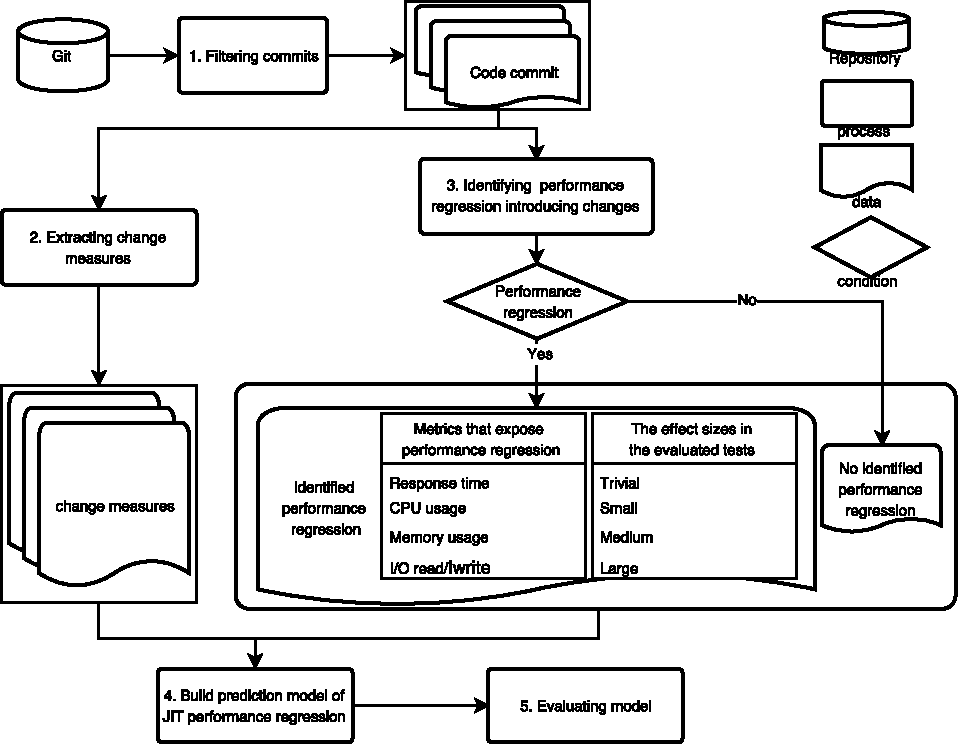
\includegraphics[width=0.85\textwidth]{workflow.pdf}
	\centering \caption{An overview of our approach that predicts performance regression introducing changes}
	\label{fig:workflow}
\end{figure*}
In general, we extract every commit and measures from the version control repositories (Git) of our subject systems and identify impacted test cases of each commit. Afterward, we evaluate performance of each commit using either the related test cases or performance micro-benchmark. Then we perform statistical analysis on the performance evaluation results to identify performance regression. Finally, we build a prediction model based on the change measures to predict the JIT performance regression introducing changes.

\subsubsection{Filtering commits}
As the first step of our approach, we start off by filtering commits in order to focus on commits that are more likely to introduce performance regressions. In particular, we use \emph{git log} command to list all the files that are changed in each commit. We only extract the commits that have source code changes, i.e., changes to \emph{$.$java} files. 

In practice, there may exist multiple commits that are made to accomplish one task, making some of the commits temporary. We would like to avoid considering the performance regressions that are introduced in such temporary commits. Since \emph{Hadoop} uses JIRA as their issue tracking system and \emph{RxJava} uses the internal issue tracking system in Github, we use the issue id that is mentioned in each commit message to identify the task of each commit. If multiple commits are associated with the same issue, we only consider the snapshot of the source code after the last commit. 
\subsubsection{Extracting change measures}
To conduct our research, we extract the domain commit-level change measures and the file-level performance-relevant change measures from the CVS repositories of the projects. The overview of the change measures is shown in Table~\ref{tab:measures}.

 \textbf{Commit-level change measures.} We consider 12 change measures grouped into five dimensions.
\begin{enumerate}[(i)]
	\item \noindent
	\textbf{Diffusion.} We use the diffusion of changes as metrics to indicate the probability that a change can introduce performance regression. In this dimension, first we investigate NS (Number of modified subsystems), ND (Number of modified directories) and NF (Number of modified files). As we introduced before, we use \textit{git log} command to get a list of changed files in current commit, each file path is divided into three parts: subsystem, directory and file, as Fig~\ref{fig:diffusion} shows, name of each subsystem is defined by the root directory name of each path, \textit{.java} file part represents the name of file, and the remaining part in the middle is used to identify the name of a directory. The correspoding measures can be conducted according to their occurance. As for Entropy, we calculate Shannon entropy using the following equations:
	\begin{equation}
		Entropy = - \sum_{i=1}^{n}\left (p_{i}\ast \log_2 p_{i} \right )
	\end{equation}
	\begin{equation}
		p_{i} =\frac{LOC\ changes\ in\ file\ i}{LOC\ changes\ in\ all\ files}
	\end{equation}
	\textit{i} means the number of files, and logarithm is used to normalize the data. Larger entropy value implies more information transmitted, which indicates more changes are caused in this context.
	
	\item \noindent
	\textbf{Size.}
	We use LOC (Lines of Code without comment line and empty lines) as metrics to evaluate the Size changes. LA (LOC added) and LD (LOC deleted) can be obtained directly from the result of \textit{git log}, and we use \textit{cloc} to get LT (LOC before the change). \textit{cloc} is an open-source project designed to count lines of source code in many programming languages. The larger size of a change,  the higher probability of introducing performance regression.
	
	\item \noindent
	\textbf{Purpose.}
	In this dimension we mainly investigate the rationale of current changes. When programmers decide to change the code, there can be different reasons like fixing bug, adding feature, improving feature, etc.
	However, bug fix sometimes can be a dangerous action because it may introduce new defects, which will also cause performance regression. In our approach, we use issue tracking systems to define whether the type of current commit is a bug fixing. We use \textit{JIRA}, a widely adopted commercial issue tracking system, to gather information about hadoop commits. Unlike hadoop, Rxjava does not have its own independent JIRA database, but we can also fetch detailed issue reports from Github for further analysis. We use scripts to crawl issue type of each commit from both JIRA and Github, because their information is authentic and up to date. Then we can determine whether a change is because of bug fixing or not.
	
	\item \noindent
	\textbf{History.}
	In History dimension, we mainly discuss two kinds of change measures: NDEV (The number of developers touched a file) and AGE (The average time interval between last and current change). Previous findings indicate that files touched by more people are more likely to introduce a problem\cite{matsumoto2010analysis}, and recent changes are easier to cause faults\cite{eick2001does}. Those unexpected deficiencies, as by-product brought by changes, are highly risky to cause performance degradations. We use \textit{git blame} command followed by touched file name, this will display who and when was each line of code touched. We count the number of different developers to obtain NDEV value. As for AGE, because we already have a list of touched files between two consecutive commits, we calculate the average time of each file and save them into a list. Because the value of time parameter is relatively large, so we need to preprocess our data before we continue our analysis.We use the following formula to normalize and rescale the data.
	\begin{equation}
		AGE = \frac{T_{Avg}-T_{Min}}{T_{Max}-T_{Min}}
	\end{equation}
	The three parameters in the equation refer to the average, maximum and minimum number in previous list. 
	
	\item \noindent
	\textbf{Experience.}
	The Experience dimension is to evaluate the programmer familiarity with the system. In our study, we mainly consider EXP (Developer experience) and REXP (Recent developer experience) as important indicators to quantify programmers' experience with a system. Increasing familiarity can reduce the likelihood of making mistakes\cite{mockus2000predicting}, and experienced specialists can capture "best practice" in software design to diminish software performance problems\cite{smith2003more}. Because all of our commits are from most recent releases, we acquire information of all contributors from  \textit{Open Hub}, a public directory of open source software with up to date information. Those information contains the total number of commits to a project, and the number of commits within recent 12 months, which can act as measures to developers' experience in our study. We crawl EXP and REXP data of all the contributors from \textit{OpenHub} and save them into different local files, the next step is to match contributor information to different commits. For RxJava, first we use \textit{git log} command to acquire all the commits and name of contributors. Therefore, we can merge those results into a larger local dataset according to name matching, and we can query information of contributors from it using commits. However, the situation in hadoop is completely different. Unlike Rxjava, there exists an agency between contributors and source repository. The middle layer is called Hadoop Project Management Committe (PMC), which contains people with direct access to hadoop repository. When programmers want to make a change in hadoop, their changes will be reviewed by a PMC member to ensure the quality. If it is approved, the reviewer will submit to hadoop repository with information \textit{"Contributed by RealContributorName"}. In consequent, from git command we can hardly tell the real contributor of a commit because only the information of commiter will be shown. So we crawling names of real contributors from JIRA and query contributor experience data from local file by name matching. 
	
	
	\begin{figure}
		\centering
		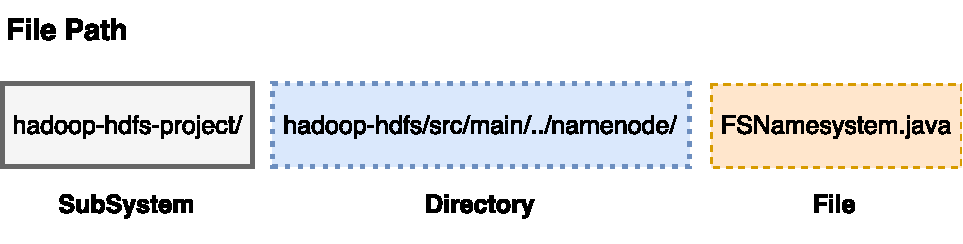
\includegraphics[width=\columnwidth]{Diffusion.pdf}
		\centering \caption{The division of file path}
		\label{fig:diffusion}
	\end{figure}
\end{enumerate}

\textbf{Performance-relevant change measures.} Simultaneously, we extract performance-relevent change measures automatically, including CC (changing conditions), CL (changing loops), FC (changing function calls), IL (Introducing locks and synchronization) and EV (expensive variables). The first three measures are most relevent to performance~\cite{ACM2016:Luo}. Also, after we find the performance regression we check the source code manully and find that IL and EV are also the most root-cause of regression. 

CC can change the code that is executed and may cause more operation eventually executed by the software, leading to performance regressions. CL may significantly slow down performance. Locks are expensive actions for software performance. IL means that introducing locks and synchronization can suspend threads waiting on a lock until released, causing performance degradation on response time. FC is that developers may introduce expensive function calls with the function execution expensive by itself or executed a large number of time. EV means that some variables are more expensive to be held in memory and need more resources to visit or operate. 

To extract performance-relevant change measures, we only need to focus on the file corresponding test case. We utilize tool \emph{srcML}~\cite{srcml_2017} to convert the source code of the same file from current commit and its parent commit to XML file. Afterward, we employ \emph{diff} tool and regular expression to compare the source code.

\begin{table}[]
	\centering
	\small
	\caption{Summary of domain and performance-relevant change measures}
	\label{tab:measures}
\begin{tabular}{|l|l|l|}
	\hline
	Dim.                         & Name    & Definition                                                                                                   \\ \hline
	\multirow{4}{*}{Diffusion}   & NS      & Number of modified subsystems                                                                                \\ \cline{2-3} 
	& ND      & Number of modified directories                                                                               \\ \cline{2-3} 
	& NF      & Number of modified files                                                                                     \\ \cline{2-3} 
	& Entropy & Distribution of modified code across files                                                                   \\ \hline
	\multirow{3}{*}{Size}        & LA      & Lines of code added                                                                                          \\ \cline{2-3} 
	& LD      & Lines of code deleted                                                                                        \\ \cline{2-3} 
	& LT      & Lines of code before the change                                                                              \\ \hline
	Purpose                      & FIX     & Whether or not the changes fix a bug                                                                    \\ \hline
	\multirow{2}{*}{History}     & NDEV    & \begin{tabular}[c]{@{}l@{}}Number of developers that changed \\ the modified files\end{tabular}              \\ \cline{2-3} 
	& AGE     & \begin{tabular}[c]{@{}l@{}}The average time interval between the \\ last and the current change\end{tabular} \\ \hline
	\multirow{2}{*}{Experience}  & EXP     & Developer experience                                                                                         \\ \cline{2-3} 
	& REXP    & Recent developer experience                                                                                  \\ \hline
	\multirow{5}{*}{Perf.} & CC      & Number of changing condition                                                                                 \\ \cline{2-3} 
	& CL      & Number of changing loop                                                                                      \\ \cline{2-3} 
	& IL      & \begin{tabular}[c]{@{}l@{}}Number of introducing locks or \\ synchronization\end{tabular}                    \\ \cline{2-3} 
	& EV      & Number of expensive variable                                                                         \\ \cline{2-3}
	& FC      & Number of changing function call                                                                             \\ \hline
\end{tabular}
\end{table}
\subsubsection{Identification of  performance regression introducing changes}
In more detail, we give a list of particular step:
%\begin{enumerate}[(i)]
%\item 

\textbf{Identifying impacted tests.} In order to evaluate performance of each code commit, we use the tests and performance micro-benchmarks that are readily available in the source code of our subject systems. As mature software projects, each subject system consist of a large amount of test cases. 
For example, \emph{Hadoop} release2.7.3 contains 1786 test cases in total. Exercising all test cases may cause two issues to our performance evaluation: 1) the test cases that are not impacted by the code change would dilute the performance impact from the code changes and introduce noise in the performance evaluation and 2) the large amounts of un-impacted test cases would requires extra resources for performance evaluation (e.g., much longer test running time). 

Therefore, in this step, we leverage a heuristic to identify impacted tests for each commit. In particular, we find that \emph{Hadoop} test cases follow a naming convention that the name of the test files contain that same name of the source code files being tested. For example, a test file named \emph{TestFSNamesystem.java} tests the functionality of \emph{FSNamesystem.java}. Hence, for each changed source code file in a commit, we automatically identify the test files. 

%\textbf{Dealing with changed tests.} Some commits may change source code and test code at the same time. Such changed test cases would bias the performance evaluation if much testing logic is added, removed or modified in the test cases. In order to minimize the impact of changed test cases in performance evaluation, we opt to use the test code before the code change, since the new version of the test cases may include new features of the system, which is not the major concern of performance regression. However, in the cases where old test cases cannot compile or failed, we use the new test cases, since the failure of the compilation or the tests indicates that the old feature may be outdated. Finally, if both new and old test cases are failed or un-compliable, we do not include this test in the performance evaluation. In total, we have 132 tests with 106 commits that use the new tests to evaluate performance and 21 test with 19 commits that are not included in our performance evaluation. There exist only six commits that are not included at all because all of their tests are either un-compliable or failed.

\textbf{Leveraging micro-benchmarks for \emph{RxJava}. }Fortunately, \emph{RxJava} provides a slew of micro-benchmarks with the goal of easing performance evaluation. We find that these performance micro-benchmarks are designed to evaluate performance of the software as a cross-cutting concern, instead of evaluating any particular features separately. Therefore, we opt to run all 76 micro-benchmarks from \emph{RxJava}. In the rest of this paper, we also refer these micro-benchmarks as test cases to ease the description of our results.

%\item 
\textbf{Evaluating performance.}
In this step, we exercise the prepared test cases and the performance micro-benchmarks to evaluate performance of each commit. We setup our performance evaluation environment based on Azure node type Standard F8s (8 cores, 16 GB memory). In order to generate statistically rigorous performance results, we adopt the practice of repetitive measurements~\cite{peterfse} to evaluate performance. 
In particular, each test or performance micro-benchmark are executed 30 times independently. We collect both domain level and physical level performance metrics during the tests. We measure the response time of each test case as domain level performance metric. A shorter response time indicating better performance of the software. We use a performance monitoring software named \emph{psutil}~\cite{psutil} to monitor physical level performance metrics, i.e., the CPU usage, Memory usage, I/O read and I/O write of the software, during the test.

%\item 
\textbf{Statistical analyses on performance evaluation.}
Statistical tests have been used in prior research and in practice to detect whether performance metric values from two tests reveal performance regressions \cite{AlGhmadi}. After having the performance evolution results, we perform statistical analyses to determine the existence and the magnitude of performance regression in a statistically rigorous manner. 
We use Student’s t-test to examine if there exists statistically significant difference (i.e., p-value $<$ 0.05) between the means of the performance metrics. A p-value $<$ 0.05 means that the difference is likely not by chance. 
A t-test assumes that the population distribution is normally distributed. Our performance measures should be approximately normally distributed given the sample size is large enough according to the central limit theorem \cite{Chen:2014}.
T-test would only tells us if the differences of the mean between the performance metrics from two commits are statistically significant. On the other hand, effect sizes quantify such differences. 

Researchers have shown that reporting only the statistical significance may lead to erroneous results (i.e., if the sample size is very large, p-value can be small even if the difference is trivial). We use \emph{Cohen\textquotesingle s d} to quantify the effects~\cite{ES2006:Becker}. \emph{Cohen\textquotesingle s d} measures the effect size statistically and has been used in prior engineering studies~\cite{IST2007:Kampenes, ICSE2002:Kitchenham}. \emph{Cohen\textquotesingle s d} is defined as:
$$
Cohen\textquotesingle s \ d=\frac{mean(x1)-mean(x2)}{s}
$$
where \emph{mean(x1)} and \emph{mean(x2)} are the mean of two populations, and s is the pooled standard deviation~\cite{JohnWiley:2011}.
$$
\mathit{effect \ size} = \left\{ \begin{array}{ll}
trivial & \textrm{if $Cohen\textquotesingle s \ d  \leqslant 0.2$}\\
small & \textrm{if $0.2 < Cohen\textquotesingle s \ d \leqslant 0.5$}\\
medium& \textrm{if $0.5 < Cohen\textquotesingle s \ d \leqslant 0.8$}\\
large& \textrm{if $0.8 < Cohen\textquotesingle s \ d$}
\end{array} \right.
$$

%\end{enumerate}
\subsubsection{Data Preprocessing}
Before utilize the attributes to build our prediction models, we need to employ data preprocessing to make sure the data quality, including accuracy, completeness, consistency and timeliness. In our project, we perform data cleaning to fill in missing values, data transformation to normalize the raw data, and remove redundant data.

Missing value happens in the \emph{FIX, EXP and REXP} in our study. Because a few commits without issue report so we cannot extract the purpose of this commit (FIX). And a few commits' contributors are not in the \emph{Hadoop} contributor official list~\cite{hadoop_2017} so we cannot calculate the measures EXP and REXP. In this case, we use a global constant to fill in the missing value. We replace all missing values by the same constant ``Unknown`` and ``1`` in measure FIX and EXP \& REXP, respectively.

Data normalization or standardization can help avoid data skew and give all measures an equal weight. The values of different attributes may have large different range due to various measurement units. It tends to give such an attribute with smaller units greater effect or weight. In particular, we perform \emph{Min-max normalization} to transform our original data.

Redundancy is an essential issue in the data integration, which means that a measure may be redundant if it is derived from another measure or a set of measures. We employ correlation analysis to remove highly correlated measures. In particular, we use \emph{Correlation-based Feature Selection} and \emph{Information Gain Rate} technique to solve this problem.

\subsubsection{Build prediction model of JIT performance regression}

\textbf{Model building.} To predict the existence of performance regression introducing change, we will build the logistic regression model (logistic regression classification can be easy to interpret) firstly to predict whether or not the change causes regression. And to predict the magnitude of performance regression introducing change, we build a ordinal model to predict the effect size of performance regression.

\textbf{Model evaluation.} We utilize two metrics to evaluate classifier performance, including \emph{precision} and \emph{recall}. It depends on confusion matrix which contains four terms consisting of \emph{true positives, true negatives, false positives and false negatives}. We perform stratified k-fold cross-validation for estimating accuracy and determine the \emph{k} as 10 due to its relatively low bias and variance.

In particular, we use the most popular machine learning tool \emph{Weka}~\cite{Hall:2009:weka} to train the dataset and build the corresponding model. Fristly we build the model and predict the text data within project. Afterward, we employ the model to predict text data cross-project.



\section{Case Study}
\label{sec:results}

Our study aims to answer three research questions. For each research question, we present 
%the motivation of the question, 
the data and approach that we use to answer the question.

\subsection*{RQ1: How well can we predict the existence of performance regression introducing change?}
%\noindent \textbf{Motivation}
%Prior research has conducted empirical studies on performance bugs \cite{Jin:2012}, using the reported performance bugs in issue reports (like JIRA issues). However, there may exist much more performance issues, such as performance regressions, that are not reported as JIRA issues. On the other hand, we evaluate performance of on each code commit instead of depending on JIRA issues. Intuitively, we may uncover instances of performance regressions that are not reported, and are not be able to investigated using the approach of prior studies. Therefore, in this research question, we start off by examining how prevalence are detected performance regression introducing changes. If we could not identify performance regressions in the subject systems, our study would be of less value to the community.

%System performance is closely related to runtime context~\cite{SIGSOFT2007:Goldsmith}. Most of the time code changes can change the runtime context so that it would have a good or bad effect on the software performance.  But It is complicated and difficult to detect the performance regression especially  in large scale system. Therefore, in this research question we want to find the performance impact of the code changes in every consecutive commits between two releases in two open source system \emph{Hadoop} and \emph{RxJava}.

 \textbf{Data and Approach}
To answer RQ1, we build a logistic regression prediction model for the risk of performance regression introducing change baesd on the commit-level and file-level measures in Table~\ref{tab:measures}. With the approach presented in Section~\ref{sec:case}, we obtain the results of performance evaluation (1 is regression, 0 is not regression) for every test case in our subject systems. In particular, we not only consider a test having performance regression if the response time is statistically significantly longer, but also think over the resource utilization. Sometimes performance regressions may not cause impact on response time but rather cause a higher resource utilization. The high resource utilization, although may not directly impact user experience, may cause extra cost when deploying, operating and maintaining the system, with lower scalability and reliability. 
%For example, systems that are deployed on cloud providers (like Microsoft Azure) may need to choose virtual machines with higher specification for higher resource utilization. Moreover, a software release with a higher memory usage is more prone to crashes from memory leaks. 
Therefore, we also use the physical metrics, i.e., CPU usage, Memory usage, I/O read and I/O write, as measurements of performance regressions. 

To validate how well the model predict performance regression introducing changes, we use two metrics, \emph{precision} and \emph{recall} to measure the model.  At the same time, to verify the stability of the prediction, we employ 10-fold cross validatoin to test the prediction model.

\jin{add data preprocess here.}

 \textbf{Results.}
We find 243 and 91 commits that contain at least one test with performance regression in at least one performance metric for \emph{Hadoop} and \emph{RxJava}, respectively. In total of 1,270 executed tests from \emph{Hadoop} and 7,600 executed tests from \emph{RxJava}, 129 and 1,410 have statistically significantly slower response time with medium or large effect sizes, respectively. When examining the effect sizes of the detected performance regressions, we find that there exist more performance-regression-prone tests with large effect sizes than medium (see Table~\ref{tab:effect}). In addition, we detect more tests with performance regressions in CPU and Memory usage, than other performance metrics. Since CPU and Memory usage both have large impact on the capacity of the software systems, these regressions may impact reliability or financial cost of the software system. 
\begin{table*}[tbh]
	\centering
	\small
	\caption{Results of identifying performance regression introducing changes in different metric classifications. }
	\label{tab:effect}
	\begin{tabular}{|c|r|r|c|r|c|r|c|r|c|r|c|r|}
		\hline
		\multicolumn{13}{|c|}{Total number of tests with performance regressions in different metrics.}                                                                                                                                                                                                                                                                                                                                                                                                                                                                                                                                                                                                                                                                                                                                                                                                \\ \hline
		\multirow{2}{*}{} & \multirow{2}{*}{\begin{tabular}[c]{@{}r@{}}Total\\ executed tests\end{tabular}} & \multirow{2}{*}{\begin{tabular}[c]{@{}r@{}}Any \\ metric\end{tabular}} & \multicolumn{2}{c|}{Response time}                                                                                                      & \multicolumn{2}{c|}{CPU}                                                                                                                & \multicolumn{2}{c|}{Memory}                                                                                                             & \multicolumn{2}{c|}{I/O read}                                                                                                           & \multicolumn{2}{c|}{I/O write}                                                                                                          \\ \cline{4-13} 
		&                                                                                 &                                                                        & \begin{tabular}[c]{@{}c@{}}large \\ effect\end{tabular} & \multicolumn{1}{c|}{\begin{tabular}[c]{@{}c@{}}medium \\ effect\end{tabular}} & \begin{tabular}[c]{@{}c@{}}large \\ effect\end{tabular} & \multicolumn{1}{c|}{\begin{tabular}[c]{@{}c@{}}medium \\ effect\end{tabular}} & \begin{tabular}[c]{@{}c@{}}large \\ effect\end{tabular} & \multicolumn{1}{c|}{\begin{tabular}[c]{@{}c@{}}medium \\ effect\end{tabular}} & \begin{tabular}[c]{@{}c@{}}large \\ effect\end{tabular} & \multicolumn{1}{c|}{\begin{tabular}[c]{@{}c@{}}medium \\ effect\end{tabular}} & \begin{tabular}[c]{@{}c@{}}large \\ effect\end{tabular} & \multicolumn{1}{c|}{\begin{tabular}[c]{@{}c@{}}medium \\ effect\end{tabular}} \\ \hline
		Hadoop            & 1,270                                                                           & 338                                                                    & \multicolumn{1}{r|}{87}                                 & 42                                                                            & \multicolumn{1}{r|}{202}                                & 97                                                                            & \multicolumn{1}{r|}{167}                                & 74                                                                            & \multicolumn{1}{r|}{75}                                 & 28                                                                            & \multicolumn{1}{r|}{75}                                 & 17                                                                            \\ \hline
		RxJava            & 7,600                                                                           & 3,100                                                                  & \multicolumn{1}{r|}{745}                                & 665                                                                           & \multicolumn{1}{r|}{659}                                & 487                                                                           & \multicolumn{1}{r|}{919}                                & 489                                                                           & \multicolumn{1}{r|}{657}                                & 449                                                                           & \multicolumn{1}{r|}{38}                                 & 0                                                                             \\ \hline
	\end{tabular}
\end{table*}

We employ our prediction model into these two systems and the result is shown in Table~\ref{tab:logistic}.

\begin{table}[]
	\centering
	\footnotesize
	\caption{Precision and recall of prediction}
	\label{tab:logistic}
\begin{tabular}{|c|c|r|c|r|c|r|c|r|}
	\hline
	\multirow{2}{*}{} & \multicolumn{2}{c|}{Runtime}                          & \multicolumn{2}{c|}{CPU}                              & \multicolumn{2}{c|}{Memory}                           & \multicolumn{2}{c|}{IO}                               \\ \cline{2-9} 
	& pre.                      & \multicolumn{1}{c|}{rec.} & pre.                      & \multicolumn{1}{c|}{rec.} & pre.                      & \multicolumn{1}{c|}{rec.} & pre.                      & \multicolumn{1}{c|}{rec.} \\ \hline
	Hadoop            & \multicolumn{1}{r|}{80\%} & 80\%                      & \multicolumn{1}{r|}{80\%} & 80\%                      & \multicolumn{1}{r|}{80\%} & 80\%                      & \multicolumn{1}{r|}{80\%} & 80\%                      \\ \hline
	Rxjava            & \multicolumn{1}{r|}{80\%} & 80\%                      & \multicolumn{1}{r|}{80\%} & 80\%                      & \multicolumn{1}{r|}{80\%} & 80\%                      & \multicolumn{1}{r|}{80\%} & 80\%                      \\ \hline
\end{tabular}
\end{table}



\subsection*{RQ2: How well can we predict the magnitude of performance regression introducing change?}

\noindent \textbf{Motivation}

In RQ1, we find that there exist prevalent performance regressions that are introduced by code changes. If we can understand what cause the introduction of these performance regressions, we may provide guidance or automated tooling support for developer to prevent the regressions during code change. 

\noindent \textbf{Approach}

We follow two steps in our approach to discover the reasons of introducing performance regressions. First, we investigate the high-level context when these performance regressions are introduced. We identify the type of issues as the context (fixing a bug or developing new features) that are related to the performance regression introducing changes. 

Second, we would like to know the code level root-causes (e.g., what kind of code change) of why the performance regressions are introduced. In particular, for each commit, we manually examine all the code changes and the corresponding test cases where performance regression are identified. We follow an iterative approach to identify the root-causes that the code change introduces performance regression, until we could not find any new reasons. 



\subsection*{RQ3: What are the important measures of performance regression introducing change?}
\textbf{Motivation.}
A lot of change measures have impact on the performance regression and Each change measure has different impact on the software quality~\cite{emadjit}. If we can find the important change measures of performance regerssion we may give the guidance to support developer to focus more on the particular factors.

\textbf{Approach.}
To address RQ3, we analyze and compare the regression coefficients of the logistic models from RQ1. To measure the effect of every change metric, we use the value of coefficients and odds ratio~\cite{Shihab:2010} in the logistic regression model. The coefficients are in fact the weights that are applied to each attribute before adding them together. We can keep all of the metrics at their original value, except for the metric whose effect we wish to measure. %We increase the value of that metric by 10\% off the original value and re-calculate the predicted probability. We then calculate the percentage of difference caused by increasing the value of that metric by 10\%. 
The effect of a metric can be positive or negative. A positive effect means that a higher value of the factor increases the likelihood, whereas a negative effect means that a higher value of the factor decreases the likelihood of the dependent variable. The odds ratio is the exponent of the corresponding coefficient in the logistic regression model. It indicates how large of an influence a change to that value will have on the prediction. We will compare the two indices and find the more important measures, and try to interpret why the measures are more important.

\textbf{Results.} \textbf{Change measure in the dimension of \emph{size} are more important than other dimension of change measures in the commit-level metrics. LA are more important change measure in the dimension of \emph{size}.} The result of  coefficients is shown in Table~\ref{tab:important}. Due to limited space, we only show the top three coefficients and odds ratios with the coresponding measures. Size dimension plays an risk-increasing role in the performance regression introducing changes. The finding is similar to prior research. Measures LT and LA in the dimension of size are more important than other measures. 

We also find that  the risk-increasing measures are different between different performance counters. In the domain level metric of \emph{Runtime}, the change measure \emph{AGE} is more important than other measures except the \emph{size} change measures. However, in the physical metrics, the performance-relevant change measures such as \emph{Loop} and \emph{Syn} are more important. So the important change measures depend on the performance conter class.

\begin{table}[]
	\centering
	\footnotesize
	%\small
	\caption{Coeffients and odds ratio with the corresponding measures in the logistic regression model.}
	\label{tab:important}
\begin{tabular}{|c|c|r|r|r|r|}
	\hline
	\multicolumn{2}{|c|}{}                                                                             & \multicolumn{1}{c|}{Runtime} & \multicolumn{1}{c|}{CPU} & \multicolumn{1}{c|}{Memory} & \multicolumn{1}{c|}{IO} \\ \hline
	\multirow{6}{*}{\begin{tabular}[c]{@{}c@{}}Coeffi\\ cients\end{tabular}} & \multirow{3}{*}{Hadoop} & AGE(2.39)                    & LD(0.40)                 & LT(0.74)                    & LT(1.38)                \\ \cline{3-6} 
	&                         & LD(1.47)                     & En.(0.17)                & LD(0.63)                    & LA(1.15)                \\ \cline{3-6} 
	&                         & LA(1.04)                     & Syn(0.15)                & Loop(0.57)                  & Loop(0.19)              \\ \cline{2-6} 
	& \multirow{3}{*}{Rxjava} & LD(0.74)                     & Syn(0.48)                & LD(1.29)                    & Fix(0.07)               \\ \cline{3-6} 
	&                         & Syn(0.18)                    & En.(0.45)                & Syn(0.21)                   & Loop(0.03)              \\ \cline{3-6} 
	&                         & Fix(0.09)                    & Fix(0.38)                & En.(0.13)                   & En.(0.02)               \\ \hline
	\multirow{6}{*}{\begin{tabular}[c]{@{}c@{}}Odds\\ ratio\end{tabular}}    & \multirow{3}{*}{Hadoop} & AGE(10.6)                    & LD(1.49)                 & LT(2.11)                    & LT(3.97)                \\ \cline{3-6} 
	&                         & LD(4.35)                     & En.(1.19)                & LD(1.87)                    & LA(3.18)                \\ \cline{3-6} 
	&                         & LA(2.84)                     & Syn(1.13)                & Loop(1.71)                  & Loop(1.19)              \\ \cline{2-6} 
	& \multirow{3}{*}{Rxjava} & LD(2.22)                     & Syn(1.62)                & LD(3.64)                    & Fix(1.07)               \\ \cline{3-6} 
	&                         & Syn(1.18)                    & En.(1.51)                & Syn(1.23)                   & Loop(1.02)              \\ \cline{3-6} 
	&                         & Fix(1.09)                    & Fix(1.41)                & En.(1.12)                   & En.(1.02)               \\ \hline
\end{tabular}
\end{table}

\textbf{Loop and Syn is more important other change measures in the dimension of performance-relevant meteics.}
Our study focused on performance regression and 

\fbox{\parbox{23.5em}{ \emph{ Our predictor achieves an average precision of 54\% percent and recall of 66\% percent. We find that there exist more performance-regression-prone tests with large effect sizes than medium. Our predictor performs better in the large effect than medium effect on performance regression.}}}







%\section{Implications of Our Findings}
%\label{sec:imp}
%\input{imp}

\section{Threat to Validity}
\label{sec:threats}
\subsection{External Validity}

\textbf{Generalizing our results. }In our case study, we only focus on fifteen releases from two open source systems, i.e., \emph{Hadoop} and \emph{RxJava}. Both of the subject systems are mainly written in \emph{Java} languages. Some of the findings might not be generalizable to other systems or other programming languages. Future studies may consider more releases from more systems and even different programming languages (such as C\#, C++). 

\subsection{Internal Validity}

\textbf{Selection of performance metrics.} Our approach requires performance metrics to measuring performance. In particular, we pick one commonly used domain level and four commonly used physical level performance metrics based on the nature of the subject systems. There exist a large number of other performance metrics. However, practitioners may require system-specific expertise to select an appropriate set of performance metrics that are important to their specific software. Future work can include more performance metrics based on the characteristic of the subject systems. 

\textbf{Model validation.}

\subsection{Construct Validity}

\textbf{Monitoring performance of subject systems.} Our study is based on the ability to accurately monitor performance of our subject systems. This is based on the assumption that the performance monitoring library, i.e. \emph{psutil} can successfully and accurately providing performance metrics. This tool monitoring library is widely used in performance engineering research~\cite{peterfse,tarekmsr16}. To further validate our findings, other performance monitoring platforms (such as PerfMon~\cite{perfmon}) can be used. 





\section{Conclusion}
\label{sec:conclusion}
Prior study of JIT defect prediction focuses more on the risk of commit based on bug rather than performance regressions. In our project, we conduct an empirical study on the JIT prediction of performance regression introducing code changes  in two open source software \emph{Hadoop} and \emph{RxJava}. To build a change risk model to predict JIT performance regression, we combine the basic commit-level measures, such as the number of modified subsystems and the purpose of the code change, with the performance-relevant measures we added, such as changing conditions and introducing synchronization. In particular, this paper makes the following contributions:
\vspace{-0.2cm}
\begin{itemize} \itemsep 0em
\item To the best of our knowledge, our work is the first to predict performance regressions at the commit level. 
\item We propose a statistically rigorous approach to identifying performance regression introducing code changes. Further research can adopt our methodology in studying performance regressions.
\item We find that change measures in dimension \emph{Size} are more risk-inceasing factors. Change measures \emph{Loop} and \emph{Synchronization} are more likely to cause performance regression.
\end{itemize}


\bibliographystyle{IEEEtran}
\bibliography{bibliography} 


% that's all folks
\end{document}


